%%%%%%%%%%%%%%%%%%%%%%%%%%%%%%%%%%%%%%%%%%%%%%%%%%%%%%%%%%%%%%%%%%%%%%%%%
% This file is part of the LaTeX sources of the OMDoc 1.3 specifiation
% Copyright (c) 2006 Andrea Kohlhase
% This work is licensed by the Creative Commons Share-Alike license
% see http://creativecommons.org/licenses/by-sa/2.5/ for details
\svnInfo $Id: cpoint.tex 8453 2009-08-04 09:58:26Z kohlhase $
\svnKeyword $HeadURL: https://svn.omdoc.org/repos/omdoc/branches/omdoc-1.3/doc/spec/projects/cpoint/cpoint.tex $
%%%%%%%%%%%%%%%%%%%%%%%%%%%%%%%%%%%%%%%%%%%%%%%%%%%%%%%%%%%%%%%%%%%%%%%%%

\section[CPoint]{{\cpoint}: An {\omdoc} Editor in MS PowerPoint}
\def\cpauthor{\scsys{CPointAuthor}}
\def\cpstudent{\scsys{CPointStudent}}
\def\cpbasic{\scsys{CPointBasic}}
\def\cpgraphs{\scsys{CPointGraphs}}
\def\cpimport{\scsys{CPointImport}}
\def\cpnotes{\scsys{CPointNotes}}
\def\texpoint{\scsys{TexPoint}}

\begin{project}{cpoint}{http://kwarc.eecs.iu-bremen.de/software/CPoint/}
\pauthors{Andrea Kohlhase}
\pinstitute{Digital Media in Education (DiMeB), Dept. of Mathematics and Computer Science, University Bremen}
\end{project}

{\cpoint} is an invasive, semantic {\omdoc} editor in MS PowerPoint (with an {\omdoc}
outlet) that enables a user to distinguish between form and content in a document. As such
it can be viewed as an authoring tool for {\omdoc} documents with a focus on their
presentational potential. It enables a user to make implicit knowledge explicit. Moreover,
it provides several added-value services to a content author in order to alleviate the
short term costs of semantic mark up in contrast to its long term gains.

\subsection{The {\cpoint} Approach}\label{sec:background}
{\cpoint} started out as a part of the Course Capsules Project
({\ccaps}) at Carnegie Mellon University (2001 --- 2004), has been subsequently supported by the
International University Bremen (2004) and is now developed further at the '{\indextoo{Digital
    Media in Education}}' group at Bremen University. {\cpoint} is distributed under
the Gnu Lesser General Public License (LGPL)~\cite{LGPL}.  The newest version can be
downloaded from the project homepage.

PowerPoint ({\ppt}) slides address exclusively the issue of {\indextoo{presentation}} ---
the placement of text, symbols, and images on the screen, carefully sequenced and possibly
animated or embellished by sound. This directly leads to the question: {\emph{What exactly
    is the content in a {\ppt} presentation?}}

Obviously, the text and the pictures carry content as does the textual, presentational,
and placeholder structure.  For instance the ordering of information by writing it in list
form, grouping information bubbles in one slide, or marking text as title by putting it
into a 'title' placeholder can be mapped directly onto the {\omdoc} {\element{omgroup}}
and {\element{metadata}} elements.  Unfortunately though, this content exploits neither
{\omdoc}'s theory level nor the statement or formula level in more than a very superficial
way.

The 'real' content is hidden beneath the presentation form: the authors, lecturers, and
audience know or learn this real content by {\bf categorizing} what they see, and {\bf
  combining} it with what they already know and presently hear. {\cpoint} stands for '{\twintoo{Content in }{PowerPoint}}'. It models this by
providing the author with a tool to explicitly store the additional {\twintoo{implicit}{knowledge}}
with the {\ppt} show itself and from within the {\ppt} environment without destroying the
presentational aspects of the {\ppt} document. Moreover, {\cpoint} {\bf converts} the
additional content to the appropriate {\omdoc} levels, so that the resulting {\omdoc}
document captures all content.  For an author the {\twintoo{semantic}{markup}} process is
a long-term investment. In order to alleviate the author's costs, {\cpoint} has
implemented several {\bf added-value services}.

\subsection{The {\cpoint} Application}\label{sec:cpoint-app}
{\cpoint} extends {\ppt}'s
presentational functionalities by semantic ones to get a handle on its visible and
invisible content. As an invasive editor (see~\cite{Kohlhase:ophcie95}) {\cpoint} makes these
{\atwintoo{semantic}{authoring}{tool}s} available through a {\indextoo{toolbar}} in the
{\ppt} menu (see {\myfigref{menubar}}) where they are available whenever {\ppt} is
running. {\cpoint} is written in Visual Basic for Applications and can be distributed as a
{\ppt} add-in.

\begin{myfig}{menubar}{The {\cpoint} Menu Bar}
  
\includegraphics[width=11cm]{projects/cpoint/CPointMenuBar}
\end{myfig}

The top-level structure of a {\ppt} presentation is given by slides.  Each slide contains
{\bf {\ppt} objects}, e.g. text boxes, shapes, images, or tables. These objects carry
certain properties like text structure (e.g. ordered lists), document structure
(e.g. being a title in the text hierarchy), or presentational structure (e.g. color, bold
font, italic font, or symbol font). {\cpoint} enables the author to attach additional
information to each {\ppt} object. In particular, the author is empowered to transform
implicit into explicit knowledge by categorizing, combining and enhancing these objects semantically.

\paragraph{Categorizing}\label{sec:annotationform}
The semantic annotation process typically starts with understanding an object's role in
the to be transmitted knowledge and a subsequent categorization. The author selects the
respective {\ppt} object and assigns a suitable (didactic) role and category from a
pre-defined list ranging from hard core mathematical categories like ``Theory'',
``Definition'', or ``Assertion'' to didactic elements like ``Question'' or ``Comment''. If a {\ppt} object is part of a
multi-part presentation (e.g. ranging over multiple slides) of a semantic entity, it can
be marked as a sequel and inherits all information from previous parts. This way the
{\ppt} dependant linearity of the objects can be overcome.

\paragraph{Combining}\label{sec:detailsform}
For categorized {\ppt} objects the author can input category specific content via the
respective details form (see {\myfigref{Content}} as an example for a {\ppt} group
categorized as ``Axiom''). In particular, {\ppt} objects can be assigned a relation via
{\cpoint}'s reference system. For instance, the axiom in {\myfigref{Content}} sits in the
theory called `taxonomy of shapes'. A more sophisticated example would be a proof
{\emph{for}} an assertion that is constructed out of several, individual proof steps
succeeding one another.  Frequently, an author wants to reference implicit knowledge (e.g.
theories can comprise entire concepts and as such are typically not explicitly presented
in a lecture). Here, she can use {\cpoint} to create abstract {\ppt} objects called {\bf
  abstract objects} that are invisible in the actual {\ppt} show but can be dealt with like all other {\ppt} objects.

\begin{myfig}{Content}{The {\cpoint} Content Form for an Axiom Object}
  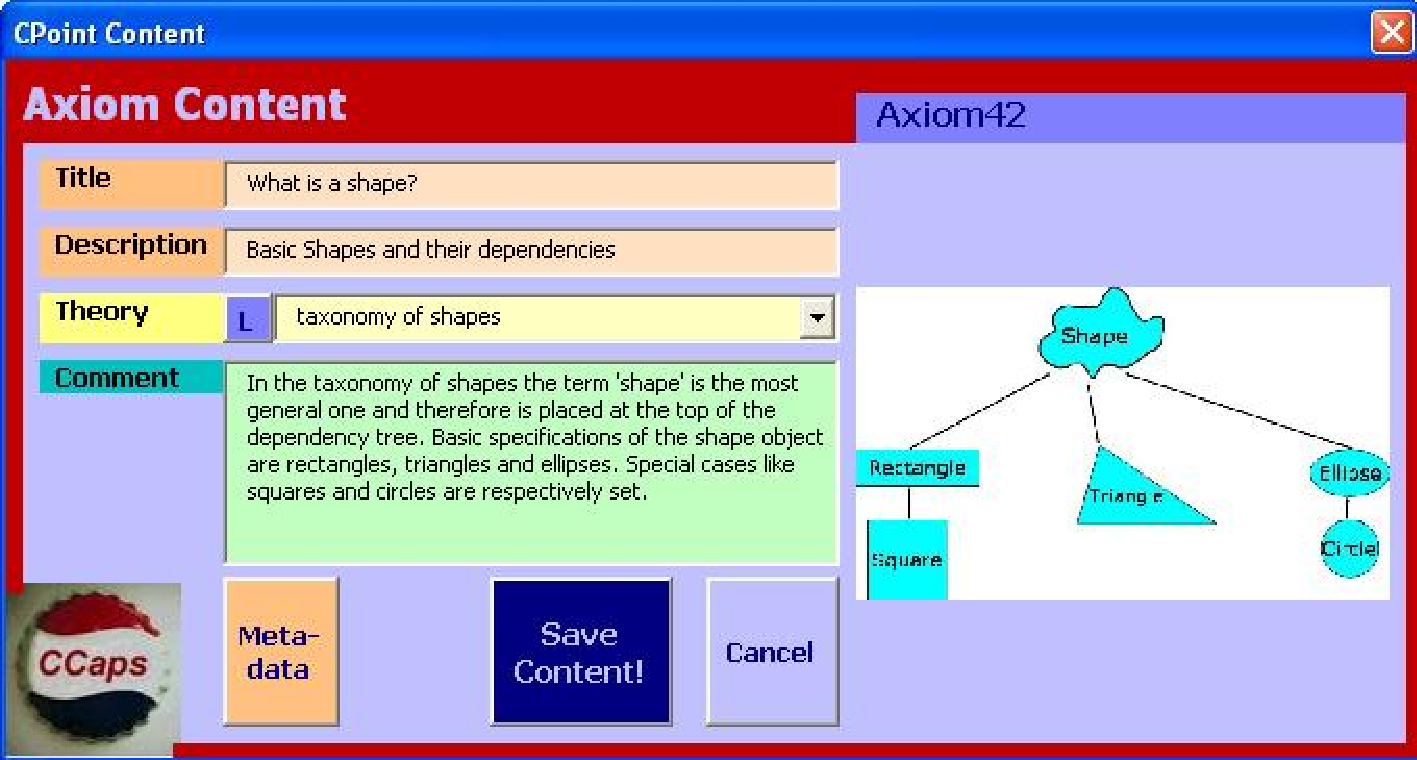
\includegraphics[width=9cm]{projects/cpoint/CPointContent}
\end{myfig}
The information annotated in these processes can be exploited for
added-value services.

\paragraph{{\omdoc} Conversion}\label{sec:omdocize} The heart of {\cpoint} is the
functionality for converting a fully ({\cpoint}-)edited presentation into a valid {\omdoc}
document.  This generated {\omdoc} document can for instance be read into
computer-supported education systems like {\activemath} (see~\cite{activemathAIEDJ01} and
{\mysecref{activemath}}).

\paragraph{Added-Value Services}\label{sec:auxiliaries}
As author support is essential for the motivation doing the semantic markup process,
{\cpoint} offers the following added-value services:
\begin{description}
\item[{\bf{Content Search and
      Navigation}\twin{content}{search}\twin{content}{navigation}}] {\cpoint}'s
  {\scsys{GoTo}} facility makes use of the additional semantic quality of {\ppt} objects
  by offering content search. For instance if an author remembers the existence of a
  definition of ``equivalence'' in some (older) {\ppt} presentation, she might look up all
  {\ppt} objects in a collection of several {\ppt} presentations that are categorized as
  ``Definition'' and whose title contain the word ``equivalence''. The author is offered a list
  of all these objects and by selecting one she is directed to the specific {\ppt} object.
\item[{\bf Dependency Graphs}\twin{dependency}{graph}] {\cpgraphs} enables the user to
  view graph based presentations of the annotated knowledge on distinct detail levels.
\item[{\bf Semantics-Induced Presentation}\twin{semantics-induced}{presentation}] The
  module {\cpauthor} offers the presentation of the underlying semantics. Whenever the
  author selects a {\ppt} object basic semantic information (like category, title, and
  main references) is presented to her. With {\cpoint}'s Visualize Mode semantic labels
  for annotated {\ppt} objects are generated.
\item[{\bf Creation of Pre-Categorized {\ppt} Objects}] Based on an individually designed
  CSS style sheet categorized, styled {\ppt} objects can be {\emph{created}} with
  {\cpauthor}. The layout is determined in the CSS file by the respective category (e.g.
  proposition) or superordinate classification (e.g. assertion, content, general).
\item[{\bf Math Glyphs in {\ppt}}\twin{mathematical}{glyph}] Based on the {\ppt} add-in
  {\texpoint}, the CMath functionalities empower an author to define individual symbol
  presentations. {\cpoint} introduces a mathematical user interface, which fully
  integrates mathematical symbols into PowerPoint presentations based on the semantics of
  the underlying objects rather than simply generating appropriate ink marks. For
  instance, the author might categorize a {\ppt} object as a symbol with the name 'reals'
  for the real numbers. The specific Unicode character to represent the real numbers can
  be declared with {\cpoint}. Subsequently, whenever the author writes the text
  '\verb|\reals|' and activates the math mode, then this sequence of characters is
  replaced by the previously declared presentation. The symbol presentation may also be
  given in {\LaTeX} form so that {\texpoint} can transform the {\LaTeX} code into {\ppt}
  glyphs. Note that this feature is not limited to math glyphs but can be used for handy
  abbreviations (macros) as well.
\item[{\bf Editorial Notes}\twin{editorial}{note}] Treating {\ppt} presentations as
  content documents requires more editing, therefore {\cpnotes} add editorial
  functionalities like grouped editorial notes and {\indextoo{navigation}} within these.
\item[{\bf {\omdoc} To {\ppt}}] The {\cpimport} module enables the import of {\omdoc}
  documents into the {\ppt} application. According to an individual underlying CSS style sheet {\ppt}
  objects in a newly created {\ppt} presentation are generated.
\item[{\bf ActiveMath}] Integrated development environment for ActiveMath content and
  specific ActiveMath book creation for a selected {\ppt} object.
\end{description}

\subsection{Future Work}
In the future the addition of other added-value services for users is planned. We want to
shift the focus from the authoring role to the recipient role of a {\ppt} presentation,
e.g. in form of a {\cpstudent} module in accordance with the {\cpauthor} module.
Furthermore, a new, more basic and therefore more user-friendly interface for {\cpoint}
novices will be implemented. This {\cpbasic} module will try to overcome the heavily
form-oriented format of {\cpoint}. In a next step the growing of a {\cpoint} user will be
supported by offering advanced {\cpoint} utilities that will extend {\cpbasic}.
Additionally, the success of ``social software'' under the Web 2.0 paradigm like ``social
bookmarking'' gives rise to the idea of a new personal and sharable {\ppt} objects
management where the predefined categories in {\cpoint} are replaced by ``social tags''.
Another {\cpoint} project is its extension for usage by teachers in school, which
usefulness has already been established in~\cite{Kohlhase:emPowerPoint}. The newest
project at the International University of Bremen is the implementation of a
{\cpoint}-like editor for MS Word.

%%% Local Variables: 
%%% mode: latex
%%% TeX-master: "../../omdoc"
%%% End: 

% LocalWords:  CPoint CPointAuthor CPointStudent CPointBasic CPointGraphs DiMeB
% LocalWords:  CPointImport CPointNotes TexPoint cpoint LGPL omgroup metadata
% LocalWords:  activemath GoTo CMath reals ActiveMath ActiveMath menubar
